% To je predloga za poročila o domačih nalogah pri predmetih, katerih
% nosilec je Tomaž Curk. Avtor predloge je Blaž Zupan.
%
% Seveda lahko tudi dodaš kakšen nov, zanimiv in uporaben element,
% ki ga v tej predlogi (še) ni. Več o LaTeX-u izveš na
% spletu, na primer na http://tobi.oetiker.ch/lshort/lshort.pdf.
%
% To predlogo lahko spremeniš v PDF dokument s pomočjo programa
% pdflatex, ki je del standardne instalacije LaTeX programov.

\documentclass[a4paper,11pt]{article}
\usepackage{a4wide}
\usepackage{fullpage}
\usepackage[utf8x]{inputenc}
\usepackage[slovene]{babel}
\selectlanguage{slovene}
\usepackage[toc,page]{appendix}
\usepackage[pdftex]{graphicx} % za slike
\usepackage{setspace}
\usepackage{color}
\definecolor{light-gray}{gray}{0.95}
\usepackage{listings} % za vključevanje kode
\usepackage{hyperref}
\renewcommand{\baselinestretch}{1.2} % za boljšo berljivost večji razmak
\renewcommand{\appendixpagename}{Priloge}
\usepackage{amssymb}
\usepackage{amsmath}

\lstset{ % nastavitve za izpis kode, sem lahko tudi kaj dodaš/spremeniš
language=Python,
basicstyle=\footnotesize,
basicstyle=\ttfamily\footnotesize\setstretch{1},
backgroundcolor=\color{light-gray},
}

\title{Nenadzorovano modeliranje}
\author{Amon Stopinšek (63150273)}
\date{\today}

\begin{document}

\maketitle

\section{Uvod}
% V tem razdelku, ki naj bo kratek in naj obsega en odstavek z do 150
% besed, na kratko opišeš, kaj je bil cilj naloge.

V nalogi smo se lotili iskanja osamelcev in gruč. V prvem delu naloge smo
poiskali filme o katerih so si gledalci najmanj enotni. Problema smo se lotili
z izračunom variance za vsak film in p testa. V drugem delu naloge smo poiskali
filme, ki so si med seboj najbolj podobni.

\section{Podatki}

% Če je naloga zasnovana tako, da vključuje analizo izbranih podatkov, v
% tem razdelku opišeš, kakšni so ti podatki in navedeš nekaj osnovnih
% statističnih lastnosti teh podatkov. Slednje vključujejo velikost
% podatkov (na primer število primerov, število in vrsto atributov), delež
% manjkajočih podatkov, opis in porazdelitev vrednosti ciljnih
% spremenljivk, in podobno. Če si podatke pridobil sam, tu opišeš, na
% kakšen način, kje in kako.

Pri nalogi smo uporabili podatkovno zbirko
\href{https://grouplens.org/datasets/movielens/}{Movie Lens}.

\section{Metode}

% Tu opišeš, na kakšen način si rešil nalogo (tehnike in metode, ki si
% jih uporabil). Lahko vključiš tudi zanimiv del programske kode, ki
% si jo morda pri tem razvil ali pa v poročilo dodatno vključiš sliko,
% kot je na primer slika~\ref{slika1}. Vse slike in tabele, ki jih
% vključiš v poročilo, morajo biti navedene v besedilu oziroma se moraš
% na njih sklicati.
%
% \begin{figure}[htbp]
% \begin{center}
% 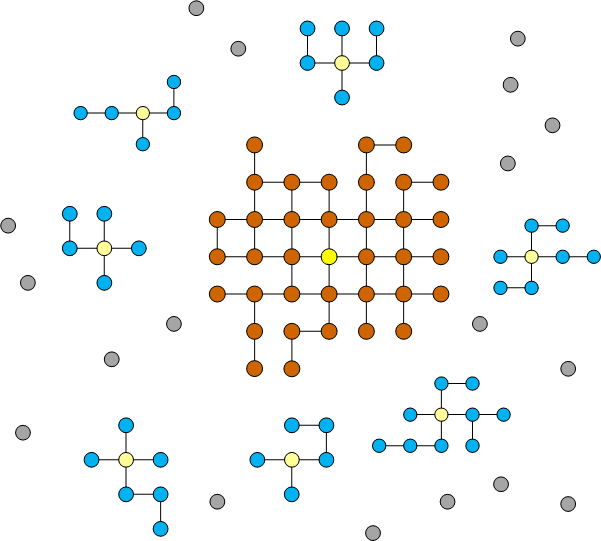
\includegraphics[scale=0.3]{slika-primer.png}
% \caption{Vsako sliko opremi s podnapisom, ki pove, kaj slika prikazuje.}
% \label{slika1}
% \end{center}
% \end{figure}
%
% V to poglavje lahko tudi vključiš kakšen metodološko zanimiv del
% kode. Primer vključitve kode oziroma implementirane funkcije v
% programskem jeziku Python je:
%
% \begin{lstlisting}
% def fib(n):
%     if n == 0:
%         return 0
%     elif n == 1:
%         return 1
%     else:
%         return fib(n-1) + fib(n-2)
% \end{lstlisting}
%
% Izris te kode je lahko sicer tudi lepši, poskušaš lahko najti še
% primernejši način vključevanja kode v Pythonu oziroma v tvojem izbranem
% programskem jeziku v okolje \LaTeX{}.

\subsection{Iskanje osamelcev}
Za iskanju osamelcev na podlagi variance ocen smo najprej preoblikovali
originalno obliko podatkov v datoteki ratings.csv v matriko\ref{tab2} kjer stolpci
predstavljajo filme, vrstice uporabnike, vrednosti pa predstavljajo oceno
filma določenega uporabnika.

\begin{lstlisting}
import pandas as pd
dfRatings = pd.read_csv('../data/ratings.csv')
df = dfRatings.pivot(index='userId', columns='movieId', values='rating')
\end{lstlisting}

\begin{table}[htbp]
\caption{Izsek iz matrike ocen}
\label{tab2}
\begin{center}
\begin{tabular}{lllllp{2cm}}
\hline
userId / movieId & 1 & 2 & 3 & 5 & 6 \\
\hline
15 & 2.0 & 2.0 & NaN & 4.5 & 4.0 \\
16 & NaN & NaN & NaN & NaN & NaN \\
17 & NaN & NaN & NaN & NaN & 4.5 \\
18 & NaN & NaN & NaN & 3.0 & 4.0 \\
19 & 3.0 & 3.0 & 3.0 & NaN & 3.0 \\
\hline
\end{tabular}
\end{center}
\end{table}

Za izračun filmov o katerih so si gledalci najmanj enotni smo uporabili varianco. Izračun variance ocen vsakega filma je bil zaradi oblike podatkov in uporabe knjižice \href{http://pandas.pydata.org/index.html}{pandas} precej preprost.

\begin{lstlisting}
df.var()
\end{lstlisting}

Pri prikazu porazdelitve izračunanih varianc so lepo porazdelitev "pokvarili"\ref{slika1}\hspace{0cm} filmi z malo ocenami. Problem smo rešili tako, da smo izločili filme z manj kot 20 ocenami.

\begin{lstlisting}
df = df.dropna(axis=1, how='any', thresh=20, subset=None, inplace=False)
\end{lstlisting}

\begin{figure}[htbp]
\begin{center}
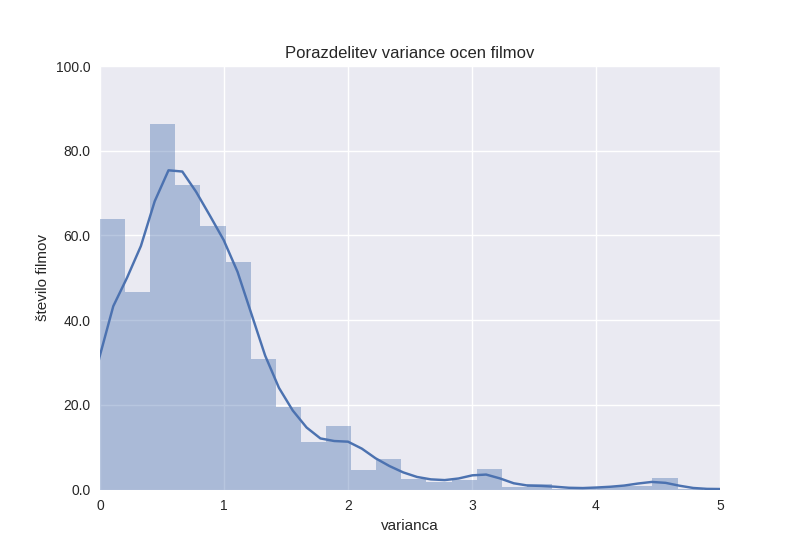
\includegraphics[scale=0.7]{porazdelitevPrva.png}
\caption{Porazdelitev variance filmov brez izločanja filmov z malo ocenami}
\label{slika1}
\end{center}
\end{figure}

\section{Rezultati}

% V tem poglavju podaš rezultate s kratkim (enoodstavčnim)
% komentarjem. Rezultate lahko prikažeš tudi v tabeli (primer je
% tabela~\ref{tab1}).

% Odstavke pri pisanju poročila v LaTeX-u ločiš tako, da pred novim
% odstavkom pustiš prazno vrstico. Tudi, če pišeš poročilo v kakšnem
% drugem urejevalniku, morajo odstavki biti vidno ločeni. To narediš z
% zamikanjem ali pa z dodatnim presledkom.

% \begin{table}[htbp]
% \caption{Atributi in njihove zaloge vrednosti.}
% \label{tab1}
% \begin{center}
% \begin{tabular}{llp{3cm}}
% \hline
% ime spremenljivke & definicijsko območje & opis \\
% \hline
% cena & [0, 500] & cena izdelka v EUR\\
% teža & [1, 1000] & teža izdelka v dag \\
% kakovost & [slaba|srednja|dobra] & kakovost izdelka \\
% \hline
% \end{tabular}
% \end{center}
% \end{table}

% Podajanje rezultati naj bo primerno strukturirano. Če ima naloga več
% podnalog, uporabi podpoglavja. Če bi želel poročati o rezultatih
% izčrpno in pri tem uporabiti vrsto tabel ali grafov, razmisli o
% varianti, kjer v tem poglavju prikažeš in komentiraš samo glavne
% rezultate, kakšne manj zanimive detajle pa vključite v prilogo (glej
% prilogi~\ref{app-res} in~\ref{app-code}).
\subsection{Iskanje osamelcev}
Na vprašanje kateri filmi imajo najbolj razpršene ocene odgovori varianca ocen posameznega filma. 

Graf\ref{slika2} prikazuje kako so porazdeljene variance ocen vseh filmov z več kot 20 ocenami.

\begin{figure}[htbp]
\begin{center}
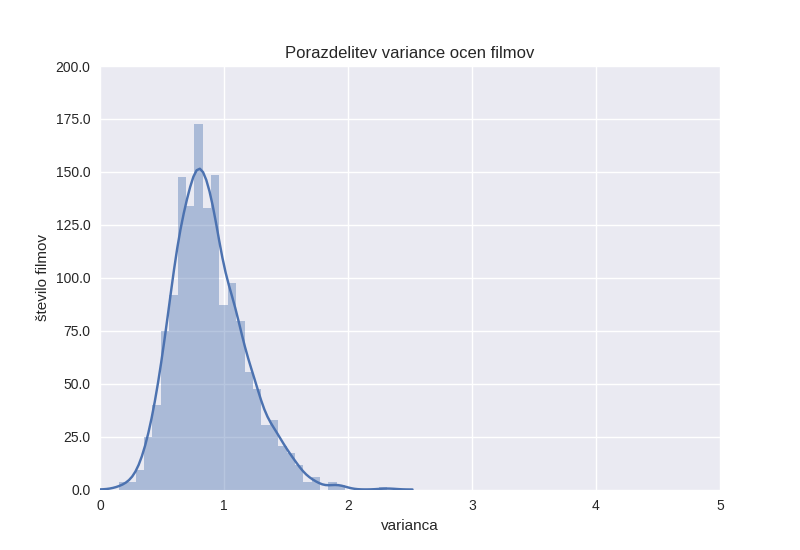
\includegraphics[scale=0.7]{porazdelitev.png}
\caption{Porazdelitev varianc ocen filmov}
\label{slika2}
\end{center}
\end{figure}

Dobljena porazdelitev zgleda precej podobna normalni. Izračunani oceni parametrov za normalno porazdelitev sta:  
\[ \mu = 0.88520202707146001 \]  
\[ \sigma^2 = 0.081338831797748562 \]  

Izračunan parametra približno opisujeta že narisano krivuljo na grafu\ref{slika2}. Za boljšo predstavo lahko
primerjamo podobnost krivulj na grafu\ref{slika2}, ki ima dorisano še krivuljo normalne porazdelitve.

Porazdelitvi se še bolje kot normalna prilega studentova porazdelitev. 

\begin{figure}[htbp]
\begin{center}
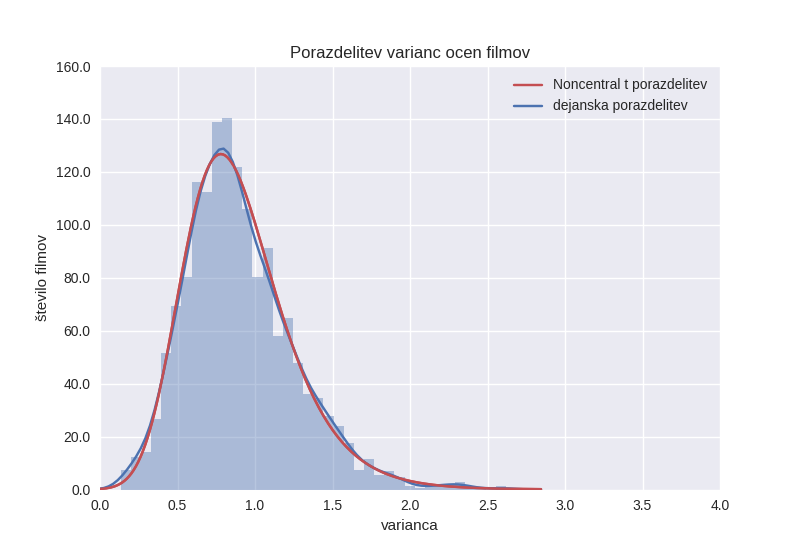
\includegraphics[scale=0.7]{porazdelitevStudent.png}
\caption{Primerjava krivulje porazdelitve s studentovo}
\label{slika4}
\end{center}
\end{figure}



\section{Izjava o izdelavi domače naloge}
Domačo nalogo in pripadajoče programe sem izdelal sam.

\appendix
\appendixpage
\section{\label{app-res}Podrobni rezultati poskusov}

% Če je rezultatov v smislu tabel ali pa grafov v nalogi mnogo,
% predstavi v osnovnem besedilu samo glavne, podroben prikaz
% rezultatov pa lahko predstaviš v prilogi. V glavnem besedilu ne
% pozabi navesti, da so podrobni rezultati podani v prilogi.

\begin{figure}[htbp]
\begin{center}
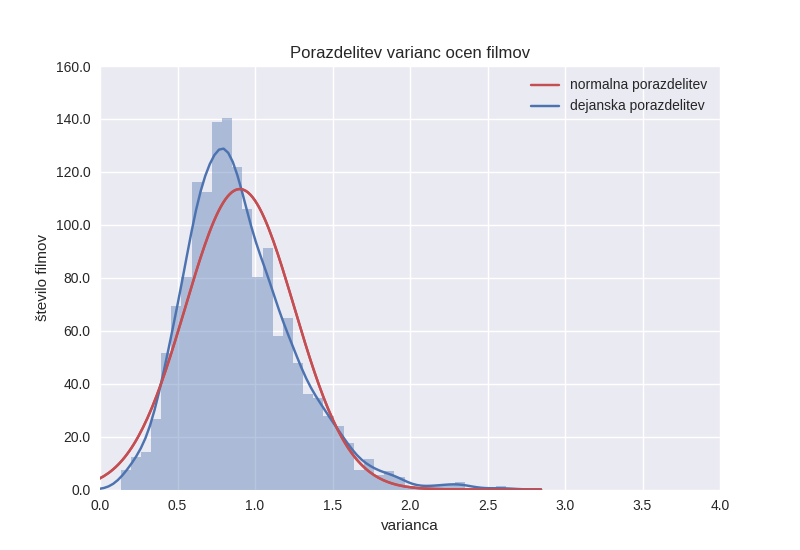
\includegraphics[scale=0.7]{porazdelitevNormalna.png}
\caption{Primerjava dejanske krivulje porazdelitve in krivulje normalne porazdelitve}
\label{slika3}
\end{center}
\end{figure}

\section{\label{app-code}Programska koda}

Za domače naloge bo tipično potrebno kaj sprogramirati. Celotno kodo oddaj
zapakirano skupaj s poročilom v datoteki zip. V kolikor je določen izsek kode
nujen za boljše razumevanje poročila, ga vključi v prilogo poročila.

Čisto
za okus sem tu postavil nekaj kode, ki uporablja Orange
(\url{http://www.biolab.si/orange}) in razvrščanje v skupine.


\begin{lstlisting}
import random
import Orange

data_names = ["iris", "housing", "vehicle"]
data_sets = [Orange.data.Table(name) for name in data_names]

print "%10s %3s %3s %3s" % ("", "Rnd", "Div", "HC")
for data, name in zip(data_sets, data_names):
    random.seed(42)
    km_random = Orange.clustering.kmeans.Clustering(data, centroids = 3)
    km_diversity = Orange.clustering.kmeans.Clustering(data, centroids = 3,
        initialization=Orange.clustering.kmeans.init_diversity)
    km_hc = Orange.clustering.kmeans.Clustering(data, centroids = 3,
        initialization=Orange.clustering.kmeans.init_hclustering(n=100))
    print "%10s %3d %3d %3d" % (name, km_random.iteration, \
    km_diversity.iteration, km_hc.iteration)
\end{lstlisting}

\end{document}
